\documentclass[12pt]{article}
%\usepackage{times}
\usepackage{cite}
\usepackage{indentfirst}
\usepackage{subcaption}
\usepackage{graphicx}
%this is a comment
\title{Volunteer Connector - Design an Implementation of your System}
\author{Daniel Domme (onid: dommed), \\
Charles Koll (onid: kollch), \\
Pedro Autran e Morais (onid: autranep), \\
Coulby Nguyen (onid: nguyenco), \\
Pavel Shonka (onid: shonkap)
}
\date{12 February 2018}

\begin{document}
\maketitle
\tableofcontents

\pagebreak
\section{UML Class Diagram}
\begin{figure}[h!]
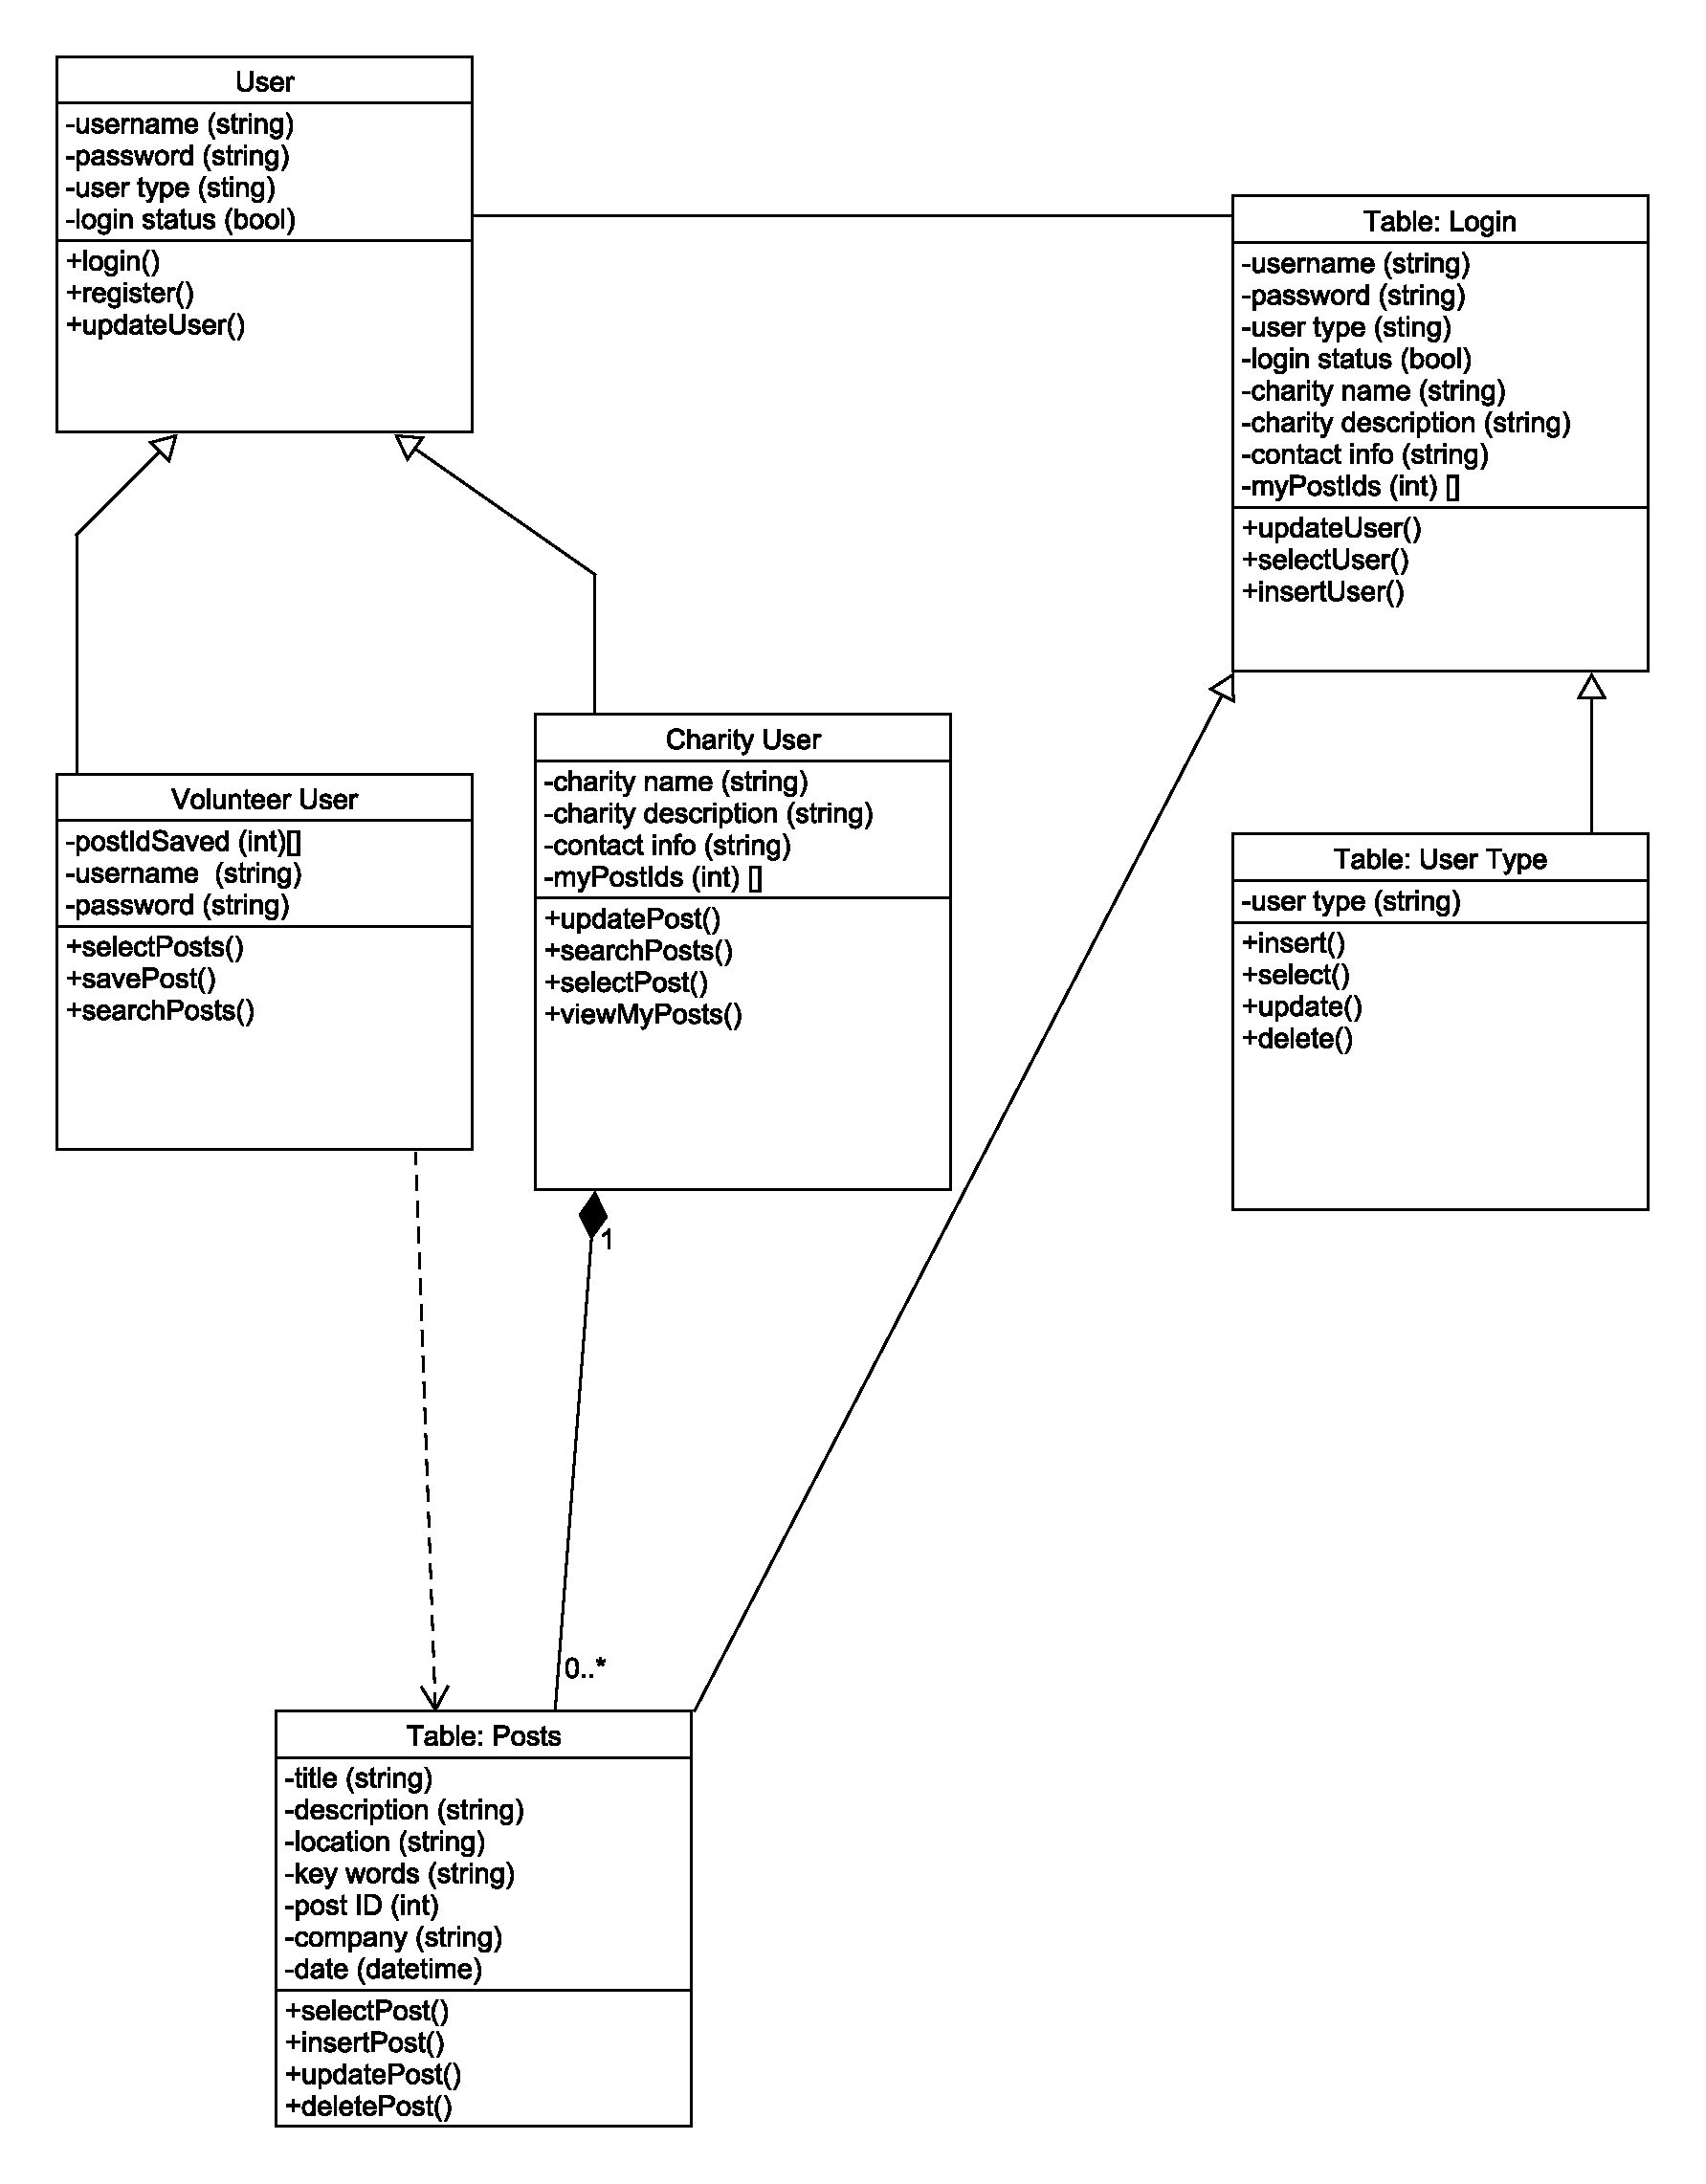
\includegraphics[width=\textwidth]{classdiagram2}
\end{figure}
\pagebreak
\section{Packages}
The User entity is closely related to the Login entity. Since the Login entity requires a
User and a User needs the Login to access the system, one cannot exist without the other.
This is clearly shown in the UML diagram by the attributes. The User's attributes
\textit{username}, \textit{password}, \textit{user type}, and \textit{login status} all
exist as attributes for the Login entity as well.

The Volunteer User and Charity User entities both have a dependency of the User entity.
Since they inherit properties from the User entity, they cannot exist if it doesn't exist.

Unlike the other entities, the Post entity does not have any dependencies and is not a
dependency for anything else. This allows it to be created at any point of the process of
building the entities.
\section{Design Patterns}
The model-view-controller design pattern would be very useful for designing our user
interface. The view in this case would be the user interface prototype we specified in our
design documents. The controller would then be the server code, probably in NodeJS, which
takes input from the view and transforms them into either commands to update the view, or
inputs to update the model, which would be a database and data storage scheme. One of the
main benefits of applying this design pattern is that it decouples the responsibilities of
each part of our web app, which allows sub-teams to work on each problem simultaneously.
Another pattern we could use is the active record pattern, which specifies how we could
access data from our relational database as objects in the model and controller parts of
our model-view-controller architecture. We can achieve this with an object-relational
mapping library. This would be a simple way to utilize the data stored in our database
from inside our server code. To make creating the user interface simpler, we might utilize
the Inversion of Control design pattern by utilizing a web framework like Express or
Rails. This allows us to separate the logic of our program from the implementation
details, letting the framework handle most of the expected code of interacting with the
network and serving data to web browser. This allows us to cut down on boilerplate code
and keep our focus on the parts of the code important to our specific app rather than the
general details of making a web app. Similarly, most of these frameworks utilize the
singleton framework by only allowing one instance of the framework to run on the server.
\section{Exceptions \& Handling}
\begin{itemize}
\item
	Exception: Due to this project heavily requiring the development team to create
	code that integrates well with each other, there might be conflicts in the code
	since different teams are creating different parts of the project.
\item
	Handler's Response: The team should respond to this problem by communicating the
	requirements that their part of the program uses, to preemptively solve
	integration issues.
\end{itemize}

\quad

\begin{itemize}
\item
	Exception: The coding of this project will likely be slowed due to project members
	being relatively new to the language and not having much experience outside of
	classes creating this sort of project.
\item
	Handler's Response: The team should respond to this problem by outsourcing to
	others for help; this could be other project members or professors. This way they
	are not coding in the dark, and will have some light that can guide them along the
	way.
\end{itemize}

\quad

\begin{itemize}
\item
	Exception: File management might be a problem if the development team are all
	commiting to the same repository, since that is where all the collaborative work
	will be done.
\item
	Handler's Response: The team should follow the instruction to work on a branch of
	the repository, instead of working on the main repository directly. This way the
	work they have completed can be reviewed and implemented into the main repository.
\end{itemize}
\section{Meeting Report}
During this week, our group managed to settle on more concrete design plans. This includes
both the structure of the code for the website/database and the actual user interface of
the website. We met a total of two times. During the first meeting, we discussed this
portion of the assignment and splitting up work, and we discussed the user interface
design. On the second meeting, we brought all of our work together and made slides for the
presentation. We then discussed what our focus will be going forward into the week. Next
week, we plan to get started on implementing the coding for the main features of the
website. We specifically would like to get the database coded and the Node.js server
working with it. We also have two more group meetings scheduled for next week. The client
was also present for the meetings.

\quad

\subsection{Contributions}
\begin{itemize}
\item
	Daniel Domme: Class Diagram, Class Diagram slide, Requirements slide, Meeting Report
\item
	Charles Koll: Packages, Latex document compilation
\item
	Pedro Autran e Morais: Design Patterns
\item
	Coulby Nguyen: Exceptions \& Handling, Sequence Diagram slide
\item
	Pavel Shonka: Planning slide
\end{itemize}
\end{document}
